\section{Analyse descriptive}\label{analyse-descriptive}

\begin{enumerate}
\def\labelenumi{\arabic{enumi}.}
\tightlist
\item
  Description de la population d'étude
\end{enumerate}

Notre population d'étude est une population assez homogène en matière
d'âge. Cependant plus on dépasse les 75 ans et moins on rencontre de
personnes. D'autres part notre popuplation est fortement masculine avec
une forte proportion des hommes quelle que soit la tranche d'âge à
l'exception des tranches du troisième âge.

\begin{figure}

{\centering 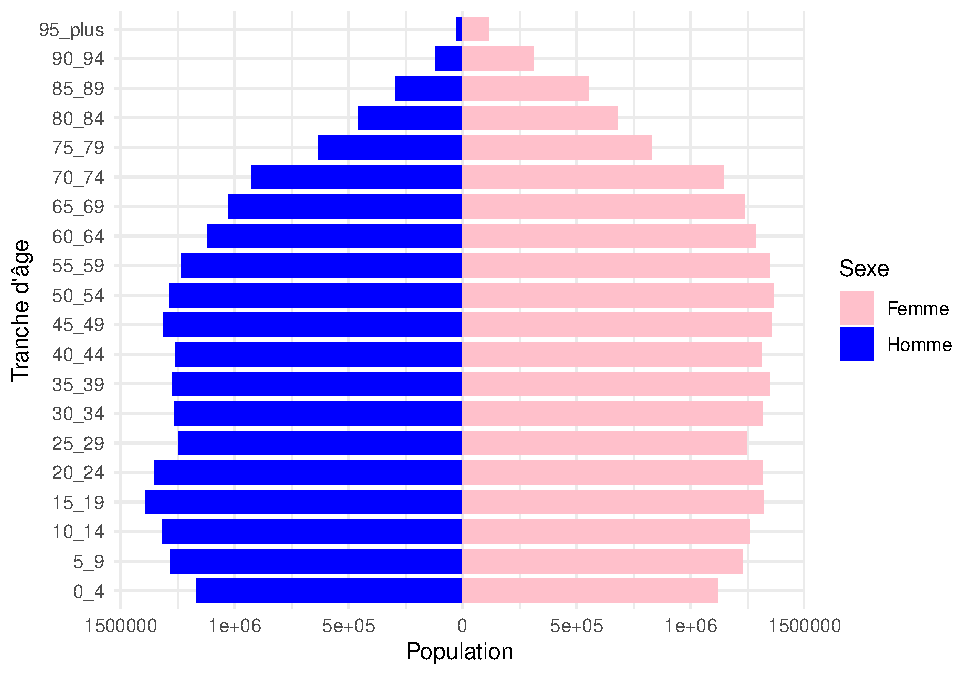
\includegraphics{4_Analyse_Descriptive_files/figure-latex/unnamed-chunk-3-1} 

}

\caption{Pyramide des âges}\label{fig:unnamed-chunk-3}
\end{figure}

Dans cette partie, nous allons réaliser quelques statistiques
descriptives sur nos données.

\subsection{Analyse univariée}\label{analyse-univariuxe9e}

\begin{enumerate}
\def\labelenumi{\arabic{enumi}.}
\tightlist
\item
  Taux et Nombre de visites
\end{enumerate}

L'analyse des statistiques descriptives sur le nombre de consultations
annuelles de médecin généraliste entre 2018 et 2022 révèle une
distribution fortement asymétrique à droite, avec une grande dispersion
des données. La moyenne de 19130 consultations, nettement supérieure à
la médiane de 9127, indique la présence de valeurs extrêmes tirant la
distribution vers le haut. Cette asymétrie est confirmée par l'écart
considérable entre le minimum de 1037 et le maximum de 765833
consultations par an.

La moitié des médecins généralistes effectuent entre 5993 et 17290
consultations annuellement, ce qui suggère une variabilité importante
dans la charge de travail. La médiane de 9127 consultations par an,
équivalant à environ 25 consultations par jour ouvrable, semble plus
représentative de l'activité typique d'un médecin généraliste que la
moyenne influencée par les valeurs extrêmes. Ces statistiques mettent en
lumière la diversité des pratiques et des charges de travail parmi les
médecins généralistes, avec potentiellement quelques cas atypiques
présentant un volume de consultations exceptionnellement élevé.

Le nombre de visites pouvant potentiellement être influencé par la
taille de la commune et donc par sa population, nous avons éliminer cet
effet en calculant le taux de consultations qui n'est autre que le
nombre de consultations moyennes par personnes.

\begin{enumerate}
\def\labelenumi{\arabic{enumi}.}
\setcounter{enumi}{1}
\tightlist
\item
  Taux de mortalité et de Natalité
\end{enumerate}

Dans les commmunes étudiées, le taux de natalité et de mortalité sont un
peu élevées avec la plupart des taux variant entre 5 et 15 pour 1000 en
ce qui concerne la natalité et 0 et 20 pour 1000 pour la mortalité. On
remarque une corrélation négative entre ces deux taux. Néanmoins cette
corrélation n'a à priori aucun sens. Par ailleurs, l'observation des
distribution permet de constater que la natalité est nde façon générale
élevée par rapport à la mortalité dans les communes étudiées.

\begin{figure}

{\centering 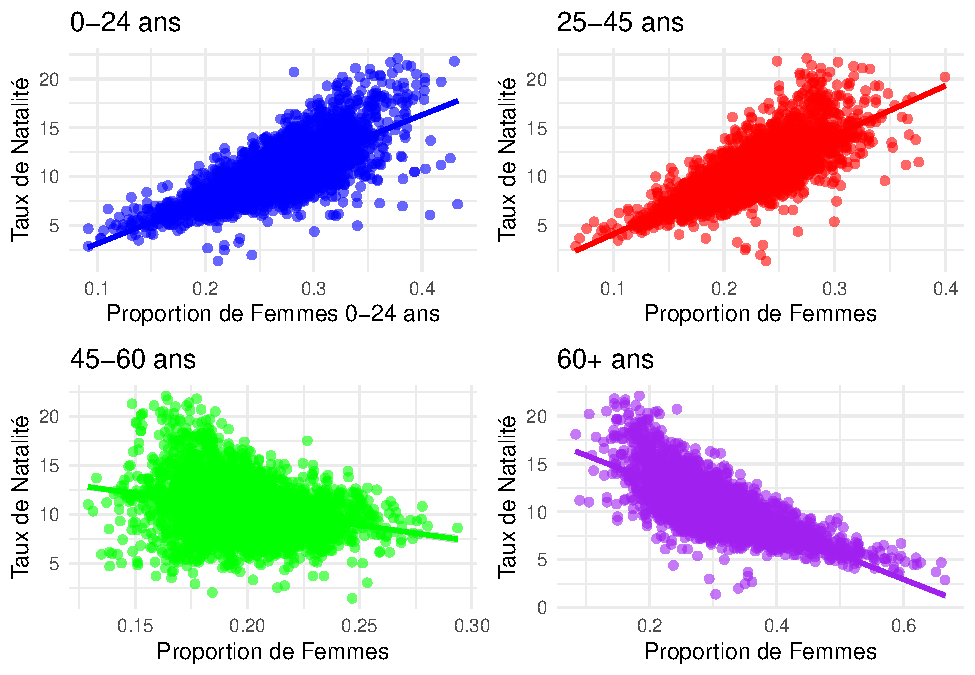
\includegraphics{4_Analyse_Descriptive_files/figure-latex/unnamed-chunk-5-1} 

}

\caption{Taux de Natalité et Taux de Mortalité}\label{fig:unnamed-chunk-5}
\end{figure}

\begin{figure}

{\centering 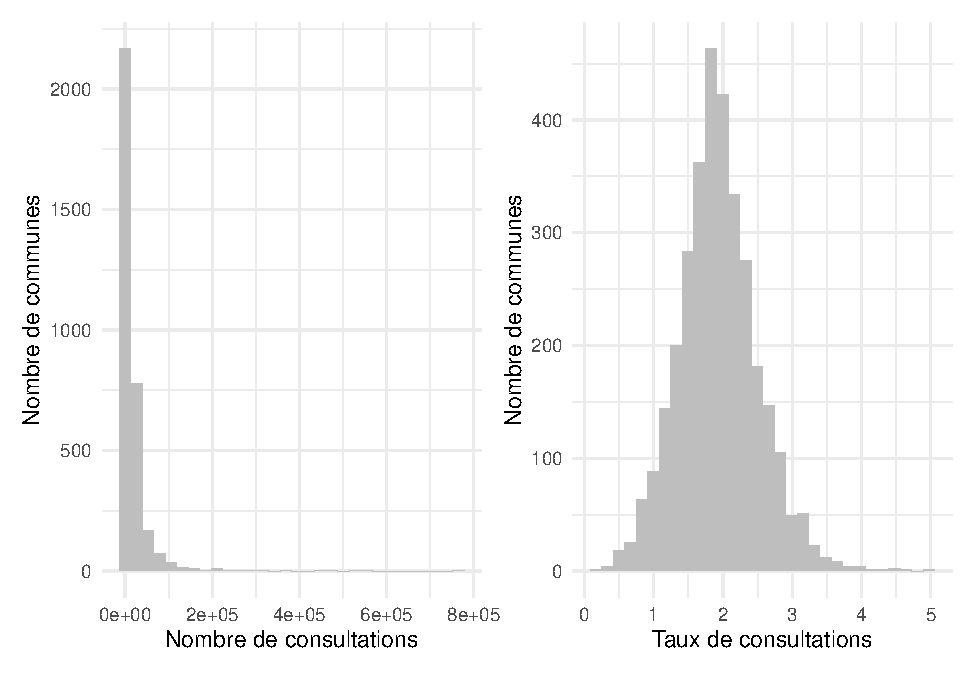
\includegraphics{4_Analyse_Descriptive_files/figure-latex/unnamed-chunk-6-1} 

}

\caption{Répartition du nombre et du taux de consultations}\label{fig:unnamed-chunk-6}
\end{figure}

\subsection{Analyse bivariée}\label{analyse-bivariuxe9e}

Nous allons ici, voir s'il y a un lien à priori entre le taux de
consultation et certaines de nos variables explicatives. Ainsi, nous
avons d'abord réalisé une analyse descriptive bivariée puis nous avons
calculé la corrélation de Pearson pour évaluer le lien linéaire entre le
taux de consulation et des variables telles que la population totale, la
part des personnes agées (75 ans et plus), la part de quelques CSP
(ouvriers et retraités).

\subsubsection{Taux de consultation et population
totale}\label{taux-de-consultation-et-population-totale}

\(\\\)

\begin{longtable}[]{@{}lr@{}}
\caption{Taux de consultations selon la taille de la
commune}\tabularnewline
\toprule\noalign{}
taille\_commune & Taux de consulations \\
\midrule\noalign{}
\endfirsthead
\toprule\noalign{}
taille\_commune & Taux de consulations \\
\midrule\noalign{}
\endhead
\bottomrule\noalign{}
\endlastfoot
Grande (\textgreater{} 8974) & 1.526810 \\
Moyenne (4849 - 8974) & 1.456356 \\
Petite (\textless= 4848) & 1.383861 \\
\end{longtable}

En divisant les communes en trois groupes égaux (ou presque égaux) en
fonction de la population totale, il ressort qu'en moyenne, plus la
taille de la commune est importante plus le taux de consulations est
élevé.

\subsubsection{Taux de consultation et population
âgée}\label{taux-de-consultation-et-population-uxe2guxe9e}

\begin{longtable}[]{@{}lr@{}}
\caption{Taux de consultations selon la population âgée}\tabularnewline
\toprule\noalign{}
population\_agee\_importante & consultations\_moyennes \\
\midrule\noalign{}
\endfirsthead
\toprule\noalign{}
population\_agee\_importante & consultations\_moyennes \\
\midrule\noalign{}
\endhead
\bottomrule\noalign{}
\endlastfoot
Non (\textless= 670) & 1.501111 \\
Oui (\textgreater{} 670) & 1.410213 \\
\end{longtable}

\begin{figure}

{\centering 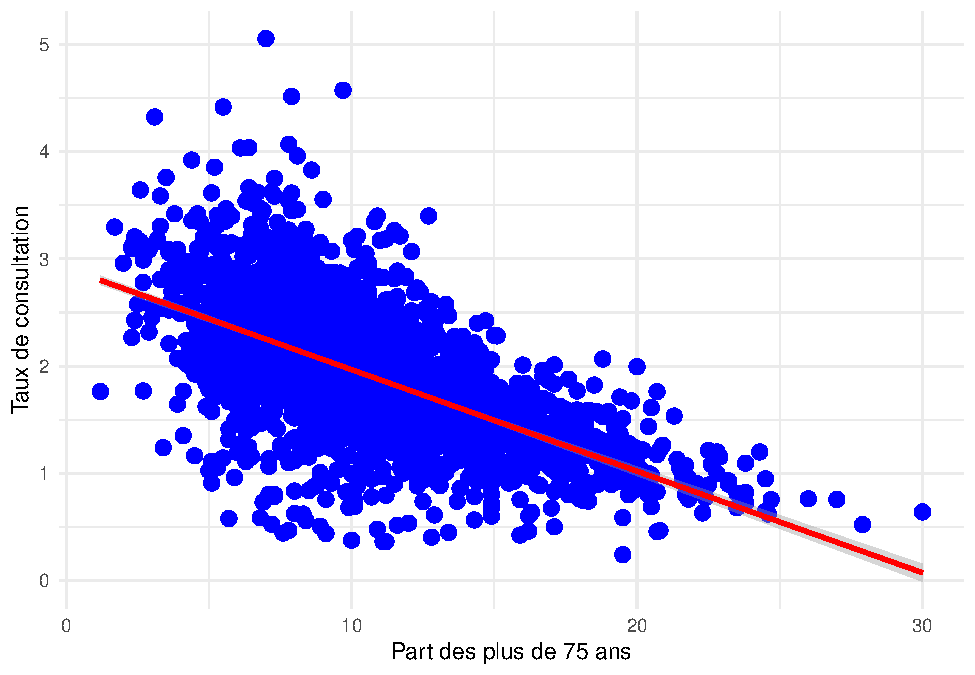
\includegraphics{4_Analyse_Descriptive_files/figure-latex/unnamed-chunk-9-1} 

}

\caption{Relation entre taux de consultations et part des plus de 75 ans}\label{fig:unnamed-chunk-9}
\end{figure}

Les communes avec une population âgée importante (communes dont la
population âgée de 75 ans ou plus est supérieure à la médiane) ont en
moyenne un taux de consultations plus faible.

\subsubsection{Taux de consultation et
CSP}\label{taux-de-consultation-et-csp}

Aucune catégorie ne semble montrer une relation linéaire évidente avec
le taux de visite. Par ailleurs, pour toutes les catégories
socio-professionnelles, la majorité des communes se situent dans une
plage de proportions faibles, ce qui limite la variabilité observable
dans les relations. Une analyse statistique supplémentaire, comme le
calcul de corrélations, serait nécessaire pour confirmer ou infirmer les
relations observées visuellement.

\subsubsection{Analyse de corrélation}\label{analyse-de-corruxe9lation}

Les résultats de la corrélation de Pearson sont consignées dans le
tableau suivant :

\begin{longtable}[]{@{}
  >{\raggedright\arraybackslash}p{(\columnwidth - 8\tabcolsep) * \real{0.0543}}
  >{\raggedright\arraybackslash}p{(\columnwidth - 8\tabcolsep) * \real{0.5652}}
  >{\raggedleft\arraybackslash}p{(\columnwidth - 8\tabcolsep) * \real{0.1304}}
  >{\raggedleft\arraybackslash}p{(\columnwidth - 8\tabcolsep) * \real{0.1087}}
  >{\raggedright\arraybackslash}p{(\columnwidth - 8\tabcolsep) * \real{0.1413}}@{}}
\caption{Corrélations de Pearson entre le taux de consultation et les
autres variables}\tabularnewline
\toprule\noalign{}
\begin{minipage}[b]{\linewidth}\raggedright
\end{minipage} & \begin{minipage}[b]{\linewidth}\raggedright
Variable
\end{minipage} & \begin{minipage}[b]{\linewidth}\raggedleft
Correlation
\end{minipage} & \begin{minipage}[b]{\linewidth}\raggedleft
P\_value
\end{minipage} & \begin{minipage}[b]{\linewidth}\raggedright
Significatif
\end{minipage} \\
\midrule\noalign{}
\endfirsthead
\toprule\noalign{}
\begin{minipage}[b]{\linewidth}\raggedright
\end{minipage} & \begin{minipage}[b]{\linewidth}\raggedright
Variable
\end{minipage} & \begin{minipage}[b]{\linewidth}\raggedleft
Correlation
\end{minipage} & \begin{minipage}[b]{\linewidth}\raggedleft
P\_value
\end{minipage} & \begin{minipage}[b]{\linewidth}\raggedright
Significatif
\end{minipage} \\
\midrule\noalign{}
\endhead
\bottomrule\noalign{}
\endlastfoot
cor & population\_municipale\_2021\_x & 0.0765022 & 0.0000118 & Oui \\
cor1 & part\_des\_pers\_agees\_de\_75\_ans\_ou\_2021 & -0.6258560 &
0.0000000 & Oui \\
cor2 & population\_de\_15\_ans\_ou\_selon\_la\_csp\_2021\_retraites &
-0.0285517 & 0.1024362 & Non \\
cor3 & population\_de\_15\_ans\_ou\_selon\_la\_csp\_2021\_ouvriers &
0.1077559 & 0.0000000 & Oui \\
\end{longtable}

Les résultats nous montrent que le taux de consultation est positivement
corrélé à la population ainsi qu'à celle de plus de 15 ans. Cependant la
corrélation est faible. Par ailleurs, la corrélation est négative avec
la part des personnes agées de plus de 75 ans. Cela dit, plus la part
des plus de 75 ans augmente moins est le taux de consultations dans une
commune. Cela peut vouloir dire que les personnes de plus de 75 ans sont
ceux qui ne se consultent pas assez.

\begin{figure}

{\centering 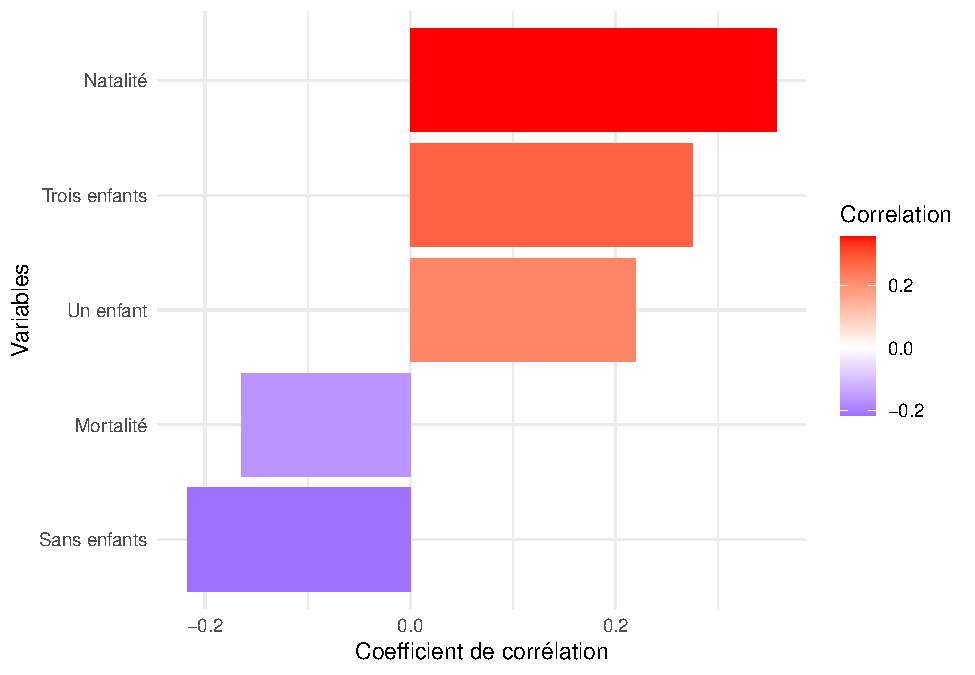
\includegraphics{4_Analyse_Descriptive_files/figure-latex/unnamed-chunk-12-1} 

}

\caption{Corrélations entre le nombre de visite et quelques variables}\label{fig:unnamed-chunk-12}
\end{figure}

\subsection{Autocorrélation}\label{autocorruxe9lation}

L'autocorrélation spatiale est une mesure essentielle pour analyser la
dépendance entre des observations géographiques. Dans notre étude nos
données sont des données portant sur des communes. Ainsi il peut exister
une dépendance entre nos taux de consultations du fait de la proximité
des communes ou de l'appartenance à un même département ou région. Ainsi
nous allons mesurer cette dépendance en évaluant l'autocorrélation
spatiale. Dans ce contexte, \textbf{l'indice de Moran} est largement
utilisé pour quantifier cette dépendance en fournissant une mesure
globale de l'autocorrélation spatiale.

\subsubsection{Définition de l'indice de
Moran}\label{duxe9finition-de-lindice-de-moran}

L'indice de Moran (\(I\)) évalue la similitude des valeurs d'une
variable entre différentes entités géographiques (par exemple, des
communes) en fonction de leur proximité spatiale. Il se base sur la
matrice de poids spatiale (\(W\)), qui définit les relations entre ces
entités.

\subsubsection{Formule de l'indice de
Moran}\label{formule-de-lindice-de-moran}

La formule mathématique de l'indice de Moran est la suivante :

\[
I = \frac{n}{\sum_{i=1}^n \sum_{j=1}^n w_{ij}} \cdot \frac{\sum_{i=1}^n \sum_{j=1}^n w_{ij} (x_i - \bar{x})(x_j - \bar{x})}{\sum_{i=1}^n (x_i - \bar{x})^2}
\]

Où :

\begin{itemize}
\item
  \(n\) : Nombre total d'entités spatiales (Ici, le nombre de communes).
\item
  \(x_i, x_j\) : Valeurs observées de la variable pour les entités \(i\)
  et \(j\) (Ici le taux de consultations)
\item
  \(\bar{x}\) : Moyenne de la variable \(x\).
\item
  \(w_{ij}\) : Poids spatial définissant la relation entre \(i\) et
  \(j\).
\end{itemize}

La matrice de \(W\) peut être constuit sur la base du voisinage entre
les deux communes ou soit de la distance entre les deux communes. Dans
le premier cas alors \(w_{ij}\) \(w_{ij} = 1\) si \(i\) et \(j\) sont
voisins et \(w_{ij} = 0\) sinon. Dans le second cas \(w_{ij} = d_{ij}\).
Nous allons dans notre cas utiliser une matrice de poids basée sur la
distance, notamment celle d'Haversine.

\subsubsection{Matrice de poids basée sur la distance de
Haversine}\label{matrice-de-poids-basuxe9e-sur-la-distance-de-haversine}

La distance de Haversine est une mesure de la distance entre deux points
sur une sphère, basée sur leurs coordonnées géographiques (\(latitude\)
et \(longitude\)). Elle est particulièrement utile pour les données
géographiques projetées sur une surface sphérique, comme la Terre.

\subsubsection{Formule de la distance de
Haversine}\label{formule-de-la-distance-de-haversine}

Si l'on considère deux points (\(i\)) et (\(j\)), la distance
(\(d_{ij}\)) entre ces deux points sur la surface d'une sphère de rayon
(\(r\)) est donnée par :

\[
 d_{ij} = 2r \cdot \arcsin\left(\sqrt{\sin^2\left(\frac{\phi_j - \phi_i}{2}\right) + \cos(\phi_i)\cos(\phi_j)\sin^2\left(\frac{\lambda_j - \lambda_i}{2}\right)}\right)
\]

Où :

\begin{itemize}
\item
  \(r\) : Rayon de la Terre (environ 6371 km).
\item
  \(\phi_i, \phi_j\) : Latitudes des points \(i\) et \(j\) (en radians).
\item
  \(\lambda_i, \lambda_j\) : Longitudes des points \(i\) et \(j\) (en
  radians). Après calcul nous avons ces statistiques sur nos distances.
\end{itemize}

Une visualtion de la densité de nos distance nous donne ceci, indiquant
une forte asymétrie à gauche de la distribution. En d'autres termes,les
communes étudiées sont assez rapprochées les unes des autres pour la
plupart.

\begin{figure}

{\centering 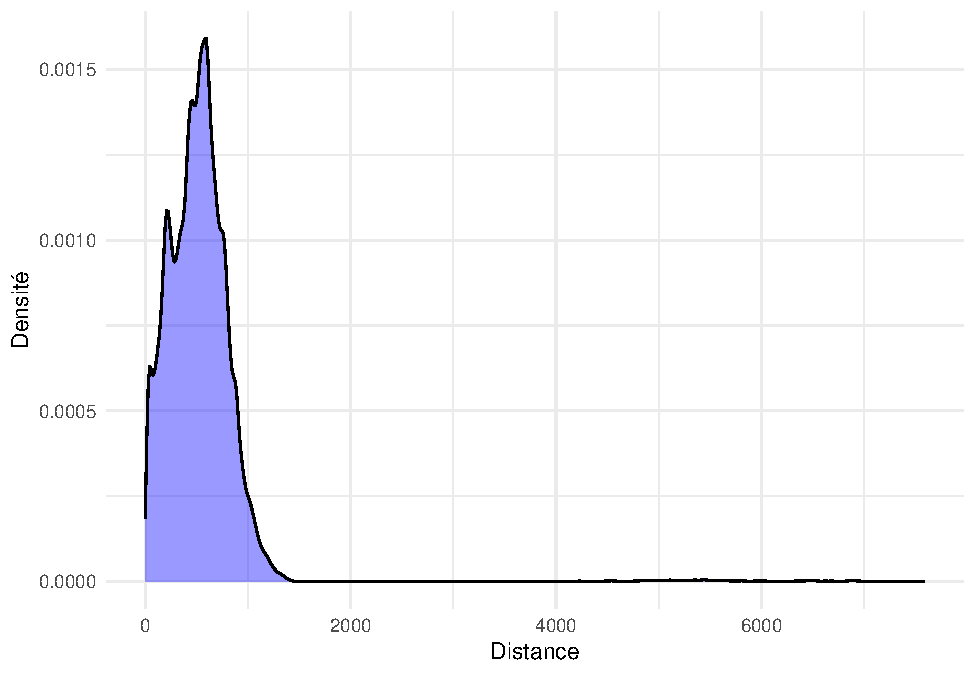
\includegraphics{4_Analyse_Descriptive_files/figure-latex/unnamed-chunk-14-1} 

}

\caption{Densité des distances}\label{fig:unnamed-chunk-14}
\end{figure}

\subsubsection{Construction de la matrice de
poids}\label{construction-de-la-matrice-de-poids}

\hfill\break
Pour construire la matrice de poids, nous avons alors suivi ces
étapes.\\

\begin{enumerate}
\def\labelenumi{\arabic{enumi}.}
\tightlist
\item
  Calculer les distances de Haversine entre chaque paire d'entités.
\item
  Définir un seuil de distance maximale (\(d_{max}\)) :

  \begin{itemize}
  \tightlist
  \item
    Si \(d_{ij} < d_{max}\), \(w_{ij} = \frac{1}{d_{ij}}\).
  \item
    Sinon, \(w_{ij} = 0\).
  \end{itemize}
\item
  Normaliser les poids pour que chaque ligne de la matrice ait une somme
  égale à 1 : \[
   w_{ij}^{norm} = \frac{w_{ij}}{\sum_{j} w_{ij}}.
  \]
\end{enumerate}

\begin{longtable}[]{@{}lr@{}}
\caption{Résultats du test de Moran}\tabularnewline
\toprule\noalign{}
& x \\
\midrule\noalign{}
\endfirsthead
\toprule\noalign{}
& x \\
\midrule\noalign{}
\endhead
\bottomrule\noalign{}
\endlastfoot
Moran I statistic & 0.1275832 \\
Expectation & -0.0003056 \\
Variance & 0.0000029 \\
\end{longtable}

Ainsi dans notre étude, nous avons trouvé un indice de Moran égale à
0.1275832. Le test nous a permi d'obtenir une p-value de 0. Ce qui
permet de conclure qu'il y a effectivement une autocorrélation positive
et significative entre les communes selon leur taux de consultations.
